\mainmatter

\chapter{Introduction}\label{introduction}

{[}Revision 4{]}

\begin{itemize}
\itemsep1pt\parskip0pt\parsep0pt
\item
  updated description of C4
\item
  updated research questions
\item
  added reference to secondary papers in research outcomes
\item
  exploitation of research results has been renamed exploitation of
  research contributions
\item
  revised description of work done abroad (section research context) and
  added figures
\end{itemize}

\section{Problem Statement}\label{problem-statement}

\reversemarginpar

This thesis is about how to improve crisis training with ICT systems.
Crisis training is an umbrella term for complex, collaborative
activities aiming at improving people's ability for \emph{preparedness}
to human and natural-caused crises (e.g.~a flood or a terrorist attack)
\autocite{Lagadec:1997js}. The term \emph{crisis} refer to a sequence of
problematic events that, if left unattended, might eventually lead to a
\emph{disaster}, causing huge damage and loss of lives. Disasters have a
huge impact on societies, both in terms of human lives and costs: over
the last 35 years, the frequency of disasters have increased five-fold;
the damage caused has multiplied by approximately eight times\footnote{Source:
  ``Council adopts new Union Civil Protection Mechanism'' Available at:
  www.consilium.europa.eu/uedocs/cmsdata/docs/pressdata/en/jha/140108.pdf.}.
According with the United Nation Office for Disaster Risk Reduction,
over the decade 1992-2012, disasters have affected 4.4 billion people
and have caused 2 trillion USD in damages worldwide\footnote{Source: The
  United Nation Office for Disaster Risk Reduction (http://unisdr.org)}.
For this reason training for better crisis management is a priority for
many countries, including the European ones.

Beside teaching the population what to do when a disaster occurs, crisis
training focuses on teaching emergency workers (e.g.~firefighters,
paramedics) how to efficiently respond to a crisis; for example by
actuating coping strategies and implementing rescue procedures (crisis
management). Each crisis is likely to be a specific, unpredictable event
that will not take place again under the same circumstances. Training
for crisis preparedness is a wicked problem, however better crisis
management can positively affect everyone's lives.

There are four main approaches to crisis training: protocol training,
tabletop exercises, physical simulations and serious games; on top of
that real crises also offer triggers for learning
\autocite{Deverell:2009fk}. In this research work we look at medium to
large scale physical simulations and serious games as key training
practices; aiming at advancing them with technology. Physical
simulations recreate at best real crises in terms of environment
(e.g.~presence of debris, collapsed buildings), and in reproducing
feelings experienced by crisis worker such as stress, tension, time
pressure and uncertainty \autocite{Borodzicz:2002em}. Yet these events
are arranged rarely. This due to the high set-up cost and the large
effort required to coordinate multiple organisations and dozens of field
workers. Moreover it has been observed that the impact of those events
is limited by lack of technologies, for example for capturing data and
maintain an overview of rescue efforts \autocite{Kyng:2006he}.
Otherwise, serious games trade the realism of physical simulations to
provide a more lightweight training experience which can be easily
reproduced frequently by single workers or teams. The ``fun'' element
typical of games is added as motivator to engage workers in frequent
play \autocite{DiLoreto:2012jj}. Physical simulation and serious games
are are not mutually exclusive but rather complementary approaches to
crisis training.

\emph{In order to maximise crisis training learning outcomes during
physical or serious game-based simulation of crisis work, training
practices already in place can be enhanced by combining (i) reflective,
experience-based learning approaches and (ii) advances in ICT and
sensing-based interaction \autocite{Zhai:2005jm}.}

Experience-based learning is a powerful tool. Facilitating learning from
work experiences of the different roles on field (e.g.~disaster managers
vs.~field workers) can bring outcomes to complement traditional formal
training. Learning from experiences entails reflection
\autocites{boud1985reflection}{Dewey:1998ug}{kolb1974toward}. Reflection
on action has been a research topic since the work of Dewey
\autocite{dewey1933we} that describes how we learn by comparing our
expectations to new and past experiences. Reflecting on action is
critical in order to learn from past experiences with the goal of
performing better in the future
\autocites{boud1985reflection}{Schon:1983ut}; and a number of tools have
been developed to support reflection, as an individual or collaborative
activity. Among those, the CSRL (Computer Supported Reflective Learning)
model developed as part of the MIRROR project\footnote{MIRROR Project -
  http://www.mirror-project.eu} aims at providing guidelines to develop
technology tools to support reflection. It identifies a cycle of four
stages of reflection \autocite{Krogstie:2013kf}: \emph{do work},
\emph{initiate reflection session}, \emph{conduct reflection session}
and \emph{apply reflection outcomes}. For each stage a number of
reflection-useful activities that can be augmented with technology are
provided.

In the context of crisis training, those activities can be summarised in
three areas: (i) capturing work experiences, (ii) re-creating work
experiences and (iii) generating realistic work experiences. Technology
provides help in different ways. Sensors can capture aspects of real or
simulated work experiences, including qualitative and quantitative
aspects; data which can be visualised on a interactive computer
interface to provide triggers for re-evaluating an experience towards a
learning outcome, or that can be used to plan new training work. Yet
current technology tools don't consider the very particular, situated
nature of crisis work. While data capturing tools lack of interaction
paradigms suitable to capture experiences \emph{in-action},
visualisation tools struggle in providing the users with context
information needed to ground the reflection \emph{on-action}. Moreover
the introduction of technology may encounter resistance in organisations
reluctant to modify accustomed practices, even if unproductive
\autocite{JCCM:JCCM15}.

Theories in the field of \emph{sensing-based interaction}, can inform
the design of novel technologies to better assist reflection in crisis
training. Sensing-based interaction is a trend in HCI which promotes
sensing information to make human-computer interfaces, -sensing-based
interfaces- more effective \autocite{Zhai:2005jm}. \emph{Tangible} and
\emph{embodied} \autocite{Dourish:2001vc} are two characterising traits
of such interfaces. They aim at enabling interaction with digital
information exploiting the affordances that everyday objects provide,
rather than traditional interaction devices such as keyboard, mouse or
touchscreens. Using sensor-based technology, conventional objects can be
augmented and turned in ``physical handles'' to digital operations
\autocite{Ishii:1997ur}, linking their traditional affordances to new
digital meanings. Making interaction with computers more ``physical''
allows for leveraging humans' skills for interaction with the real world
\autocite{Shaer:2009fx}. This approach might be well suited for crisis
field work which, contrarily to traditional office work, has a strong
physical and spatial connotation. In this perspective, tangible and
embodied interfaces have been successfully employed to provide natural
\autocite{Terrenghi:2005gq} and situated \autocite{Klemmer:2006ez}
learning and increased reflection and engagement
\autocite{Rogers:2006te}. ``Being able to move around in the world and
interact with pieces of the world enables learning in ways that reading
books and listening to words do not''. \autocite{Klemmer:2006ez}

Yet building prototypes of sensing-based interfaces, is a complex task
which requires scientists to master a wide set of skills including
product design, hybrid software and electronics development; hardware
construction and assembly. This is this still a relatively new area in
HCI and it is characterised by the absence of a widely established
toolchain to help the prototyping work. Rather it is characterised by
fast adoption of edging technologies and a pragmatic attitude at
\emph{tinkering} and \emph{thinking-thrugh-prototyping}
\autocite{Klemmer:2006ez}. Considering the essential role of prototypes
in the development of novel sensing-based interfaces; developing a
skillset to enable rapid prototyping of hybrid software/hardware
products is essential to the accomplishment of the goals sought by this
PhD work.

\begin{figure}[tbh]
    \centering
    \includegraphics[width=0.70\textwidth]{better_management}
    \caption{Relation among the three domain of this thesis}
    \label{fig:topic_relation}
\end{figure}

\section{Research methodology}\label{research-methodology}

The work in this thesis is based on \emph{design research}
\autocites{Hevner:2010fy}{March:1995gm}. The work followed a \emph{user
centred approach} \autocites{MAGUIRE:2001dp}{Gulliksen:2003hd}, based on
exploratory studies and design work in multiple iterations.

Several qualitative research methods \autocite{robson1993real} have been
adopted, including shadowing and observations of crisis workers, during
field studies and interviews. Scenarios, personas and mockups aided the
user-centred design work. Consistently with design research methodology,
grounded on the activities of \emph{building} artefacts for a specific
purpose and of \emph{evaluating} how well the artefacts perform
\autocite{March:1995gm}, a number of prototyping iterations and
evaluation studies have been performed.

Prototyping involved the construction of hardware and software ICT
systems to support reflection processes. The design of prototypes was
grounded in field studies during physical simulations of crisis I
attended. Simple prototypes were initially used to build a deeper
understanding of the crisis domain, for which I didn't have a previous
knowledge. They acted as technology probes \autocite{Hutchinson:2003il}
and facilitate building and understanding of the crisis domain by
engaging users in focus groups. Later, multiple iterations implemented a
growing set of requirements in fully working prototypes robust enough to
be deployed during simulated rescue work.

User evaluations followed each design iteration \ref{fig:cromar}. The
aim was both in assessing usability of the prototypes and relevance of
reflection outcomes they might produce. Prototypes were evaluated both
during focus groups and during large simulations of crisis response
works. Results from evaluations have fed following design iterations,
contributed in the validation of theories on reflective learning and
into the development of new constructs.

\begin{figure}[tbh]
    \centering
    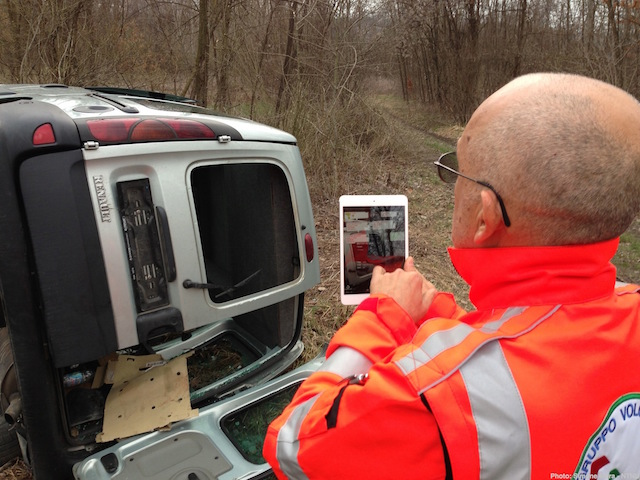
\includegraphics[width=0.85\textwidth]{introduction_cromar}
    \caption{One of the evaluation studies performed}
    \label{fig:cromar}
\end{figure}

\section{Research questions}\label{research-questions}

The main research question for the PhD work is:

\begin{quote}
MRQ: What are the opportunities introduced by combining reflective
learning theories with sensing-based interfaces for supporting crisis
training?
\end{quote}

To answer the main research question the work has been broken down into
three sub-questions:

\begin{quote}
RQ1: How sensing-based interfaces can be designed to enable unobtrusive
experience collection during crisis work?
\end{quote}

\begin{quote}
RQ2: How sensing-based interfaces can be designed to trigger reflection
via re-creation or generation of work experiences?
\end{quote}

\begin{quote}
RQ3: How sensing-based interfaces for supporting reflection can be
rapidly prototyped?
\end{quote}

While the first two questions aim at investigating the design of systems
to support with technology the tasks of \emph{capturing},
\emph{re-creating} and \emph{generating} work experiences; the third
question investigates how toolkits and open-source communities can ease
the implementation of design ideas into prototypes.

\section{Research outcomes}\label{research-outcomes}

Three are the main outcomes of this PhD work.

Seven research papers published in peer-reviewed conferences and
journals explored the research questions (Section
\ref{research-papers}).

Building on results reported in the papers, a body of knowledge
contributing in the fields of technology enhanced learning (TEL), IS for
crisis response (ISCRAM) and tangible and embodied computing (TEI) has
been developed. (Section \ref{research-contributions})

Finally research contributions have been evaluated for commercial
exploitation. Five \emph{Disclosure of Invention (DOFI)} have been filed
for technology transfer and early contacts with the industry have been
established.

\subsection{Research papers}\label{research-papers}

The research questions RQ1-RQ3 are addressed in the following research
papers:

\begin{quote}
\textbf{P1} Mora, S., Boron, A., \& Divitini, M. (2012). CroMAR: Mobile
Augmented Reality for Supporting Reflection on Crowd Management.
\emph{International Journal of Mobile Human Computer Interaction}, 4(2),
88--101.
\end{quote}

\begin{quote}
\textbf{P2} Mora, S., \& Divitini, M. (2014). Supporting Debriefing with
Sensor Data: A Reflective Approach to Crisis Training. \emph{In
Proceeding of Information Systems for Crisis Response and Management in
Mediterranean Countries, ISCRAM-MED}, 196(7), 71--84.
\end{quote}

\begin{quote}
\textbf{P3} Mora, S., \& Divitini, M. (2014). WATCHiT: a modular and
wearable tool for data collection in crisis management and training.
\emph{In Proceeding of the European Conference in Ambient Intelligence,
AMI}, 8850(22), 274-289.
\end{quote}

\begin{quote}
\textbf{P4} Di Loreto, I., Mora, S., \& Divitini, M. (2012). Don't
Panic: Enhancing Soft Skills for Civil Protection Workers. \emph{In
Proceeding of International Conference on Serious Games Development
Applications, SGDA}, 7528(1), 1--12.
\end{quote}

\begin{quote}
\textbf{P5} Mora, S., Di Loreto, I., \& Divitini, M. The
interactive-token approach to board games. \emph{Ready for submission}.
\end{quote}

\begin{quote}
\textbf{P6} Müller, L., Divitini, M., Mora, S., Rivera-Pelayo, V., \&
Stork, W. (2014). Context Becomes Content: Sensor Data for Computer
Supported Reflective Learning. \emph{IEEE Transactions on Learning
Technologies}, PP(99).
\end{quote}

\begin{quote}
\textbf{P7} Mora, S., \& Farshchian, B. A. (2010). A Unified
Architecture for Supporting Direct Tag-Based and Indirect Network-Based
Resource Discovery. \emph{In Proceeding of the International Conference
on Ambient Intelligence, AMI}, 6439(20), 197--206.
\end{quote}

Table \ref{tab:rq-papers-relation} shows the mapping between research
papers and research questions.

\begin{table}[tbh]
\centering
\caption{The relation between research papers and research questions.}
\label{tab:rq-papers-relation}
\begin{tabular}{p{\dimexpr 0.075\linewidth-2\tabcolsep}p{\dimexpr 0.40\linewidth-2\tabcolsep}ccccccc}
\toprule
\multicolumn{2}{l}{Research questions}    & P1 & P2 & P3 & P4 & P5 & P6 & P7 \\
\midrule
RQ1 & How sensing-based interfaces can be designed to enable unobtrusive experience collection during crisis work? & & \textbullet & \textbullet & & & \textbullet & \\
RQ2 & How sensing-based interfaces can be designed to trigger reflection via re-creation or generation of work experiences?  & \textbullet & \textbullet & & \textbullet & \textbullet & \textbullet & \\
RQ3 & How sensing-based interfaces for supporting reflection can be rapidly prototyped?  & & & \textbullet & & \textbullet & & \textbullet \\
\bottomrule
\end{tabular}
\end{table}

In addition to these papers, this PhD work has produced fourteen
secondary peer-reviewed publications presented in conferences and
workshops. Those works preset incremental achievements in research that
have added to the investigation of research questions. Abstracts of the
papers are included in Appendix \ref{secondary-papers}

\subsection{Research contributions}\label{research-contributions}

The seven paper published added to the following contributions of this
research work. The relation between research papers and the main topics
of the research contributions is represented in Figure \ref{fig:mapping}

\begin{quote}
\emph{\textbf{C1:} Implementation and evaluation of MIRROR Computer
Supported Reflective Learning (CSRL) theory.} It includes a validation
of previous theoretical models and in the formulation of new constructs
\end{quote}

\begin{quote}
\emph{\textbf{C2:} Knowledge about designing experience-capturing tools
for crisis workers.} It defines the design space as well as design
challenges for building computer-based data capturing tools.
\end{quote}

\begin{quote}
\emph{\textbf{C3:} Novel sensing-based interaction techniques to support
re-creation and generation of work experiences in crisis training.} It
describes novel user interfaces for the visualisation and manipulation
of data captured from working experiences.
\end{quote}

\begin{quote}
\emph{\textbf{C4:} Knowledge about implementing prototypes to be
deployed into the wild.} Drawing from the author's experience, it
presents presents challenges and lessons learnt for building prototypes
of sensing-based interfaces.
\end{quote}

\begin{figure}[tb]
    \centering
    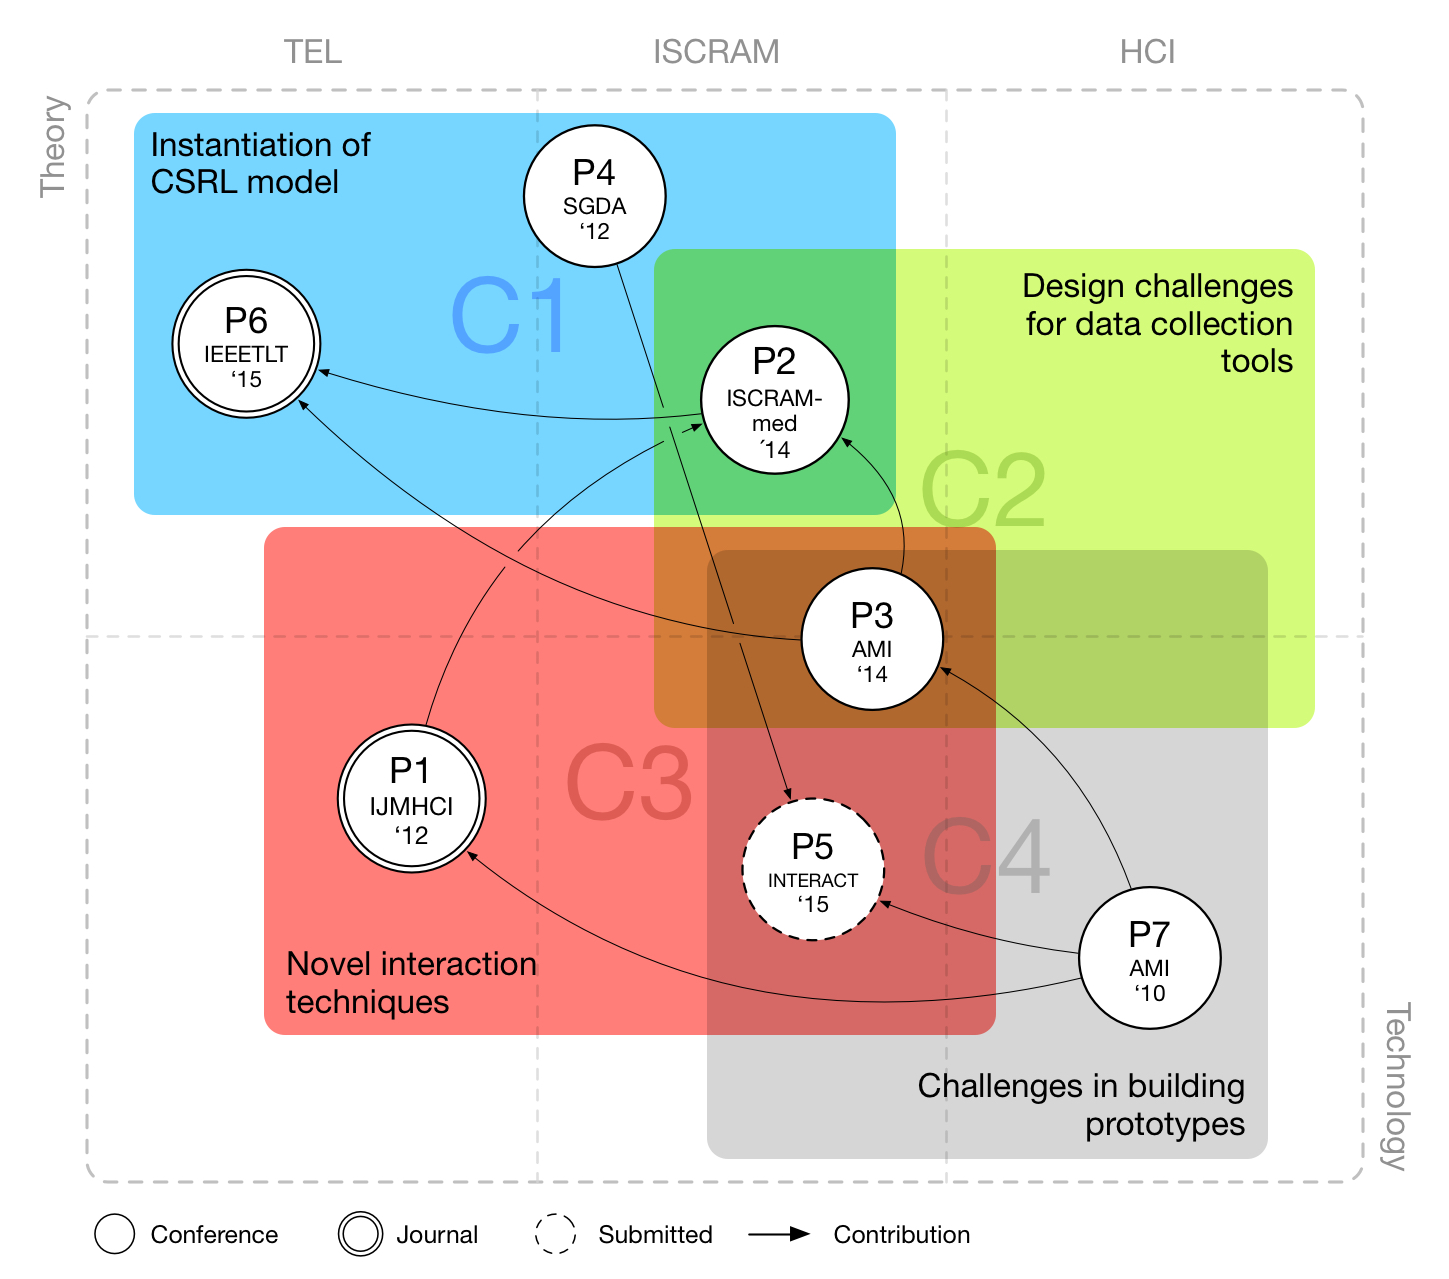
\includegraphics[width=1\textwidth]{papers-contributions-mapping}
    \caption{Research papers and the main topics of the research contributions}
    \label{fig:mapping}
\end{figure}

These contributions are relevant for several research communities
including Technology Enhanced Learning (TEL) (C1), Tangible Embodied
Embedded Computing (TEI) (C3, C4), Information systems for Crisis
Response (ISCRAM) (C1,C2)

\subsection{Exploitation of research
contributions}\label{exploitation-of-research-contributions}

During the final phase of the investigation, commercial exploitation of
research contributions has been investigated. The focus was in assessing
efforts needed and path of actions to evolve the prototypes developed as
theory demonstrator into commercial products. To this end, I co-authored
five \emph{Disclosure of Invention} (DOFI): technical documents that
capture the description of the technologies created and establish
inventor-ship. DOFIs were drafted based on information published in
research paper (Table \ref{tab:papers-inventions})

\begin{table}[tbh]
    \centering
    \caption{Relation between the invention registered and research papers}
    \label{tab:papers-inventions}
\begin{tabular}{p{\dimexpr 0.05\linewidth-2\tabcolsep}p{\dimexpr 0.30\linewidth-2\tabcolsep}p{\dimexpr 0.50\linewidth-2\tabcolsep}p{\dimexpr 0.15\linewidth-2\tabcolsep}}
\toprule
  & Authors    & Invention  &  Research papers  \\ \midrule
I1 & Mora, S., Boron, A. and Divitini, M.   & CroMAR. Situated reflection and training in crisis management.   & P1, P2    \\ \noalign{\smallskip}
I2 & Mora, A. and Divitini, M. & WATCHiT. Wearable data collection in crisis management and training & P2, P3 \\ \noalign{\smallskip}
I3 & Di Loreto, I., Mora, S. and Divitini, M. & “Don’t Panic!” A serious game for enhancing soft skills for Civil Protection workers & P4, P5 \\ \noalign{\smallskip}
I4 & Mora, S., Di Loreto, I. and Divitini, N. & Anyboard: a platform for creating and play digital board games & P5 \\ \noalign{\smallskip}
I5 & Mora, S. and Divitini, M. & TILES Toolkit. Building seamless interfaces between people and the Internet of Things & P3, P5 \\
\bottomrule
\end{tabular}
\end{table}

Disclosure of inventions were filed at the NTNU Technology Transfer
office\footnote{NTNU Technology Transfer AS - http://www.tto.ntnu.no}, a
business incubator affiliated with NTNU, in accordance with the
Norwegian law\footnote{In accordance with
  ``Arbeidstakeroppfinnelsesloven'', ``Universitets og høgskoleloven''
  and NTNU's internal Guidelines for innovation}. They were used by
technology transfer managers to assess patent applicability and
establishment of commercial activities. To this effort, I presented
research results to several subjects from the industries working in the
emergency management field, raising positive and supportive feedbacks.
In November 2014 I was granted by NTNU Discovery \footnote{NTNU
  Discovery - http://ntnudiscovery.no} a 150.000NOK
(\textasciitilde{}22.000USD) seed for financing further commercial
exploration of the research results after the PhD completion.

\section{Context of the work}\label{context-of-the-work}

The research presented in this thesis is framed within the EU-funded
(IST-FP7) project MIRROR\footnote{MIRROR Project -
  http://www.mirror-project.eu}. The focus of MIRROR is the creation of
a set of technology applications that enable employees to learn from
their own and others' experiences to perform better in the future. As an
associate researcher of MIRROR I took part in shaping the results of the
projects by designing and implementing ICT systems, writing deliverables
and attending project meetings. Thanks to MIRROR I cooperated with
crisis worker associations to run user and evaluation studies. I also
benefited from discussions and joined works and publications with
members of the consortium. After the prohect final review in September
2014, MIRROR has been graded as ``Excellent'' by the EU commission.

During the PhD I worked as visiting researcher in two foreign
institutions: City London University\footnote{City London University -
  http://city.ac.uk} in London (UK) and MIT SENSEable City Lab\footnote{MIT
  SENSEable City Laboratory - http://senseable.mit.edu} in Boston, MA
(USA). The purpose of the two visits was to investigate whether the
technologies developed during the PhD could be generalised to
application domains that share similarities with crisis training.

During fourteen weeks spent as visiting fellow at City University I
investigated the design and production of \emph{Hazel Court}, a
digitally augmented serious game for training of dementia carers for
better care. I worked under the supervision of professor Neil Maiden. A
working prototype of \emph{Hazel Court} (Figure \ref{fig:hazel-court})
has been implemented and evaluated in eight care homes in the greater
London area. The game design and underpinning theories are reported in a
joined publication to be submitted. This experience strengthened my
competences in building sensing based-interfaces to support reflection
in a domain which shares similarities with crisis training. It added to
the study of RQ2 and RQ3.

\begin{figure}[h]
    \centering
    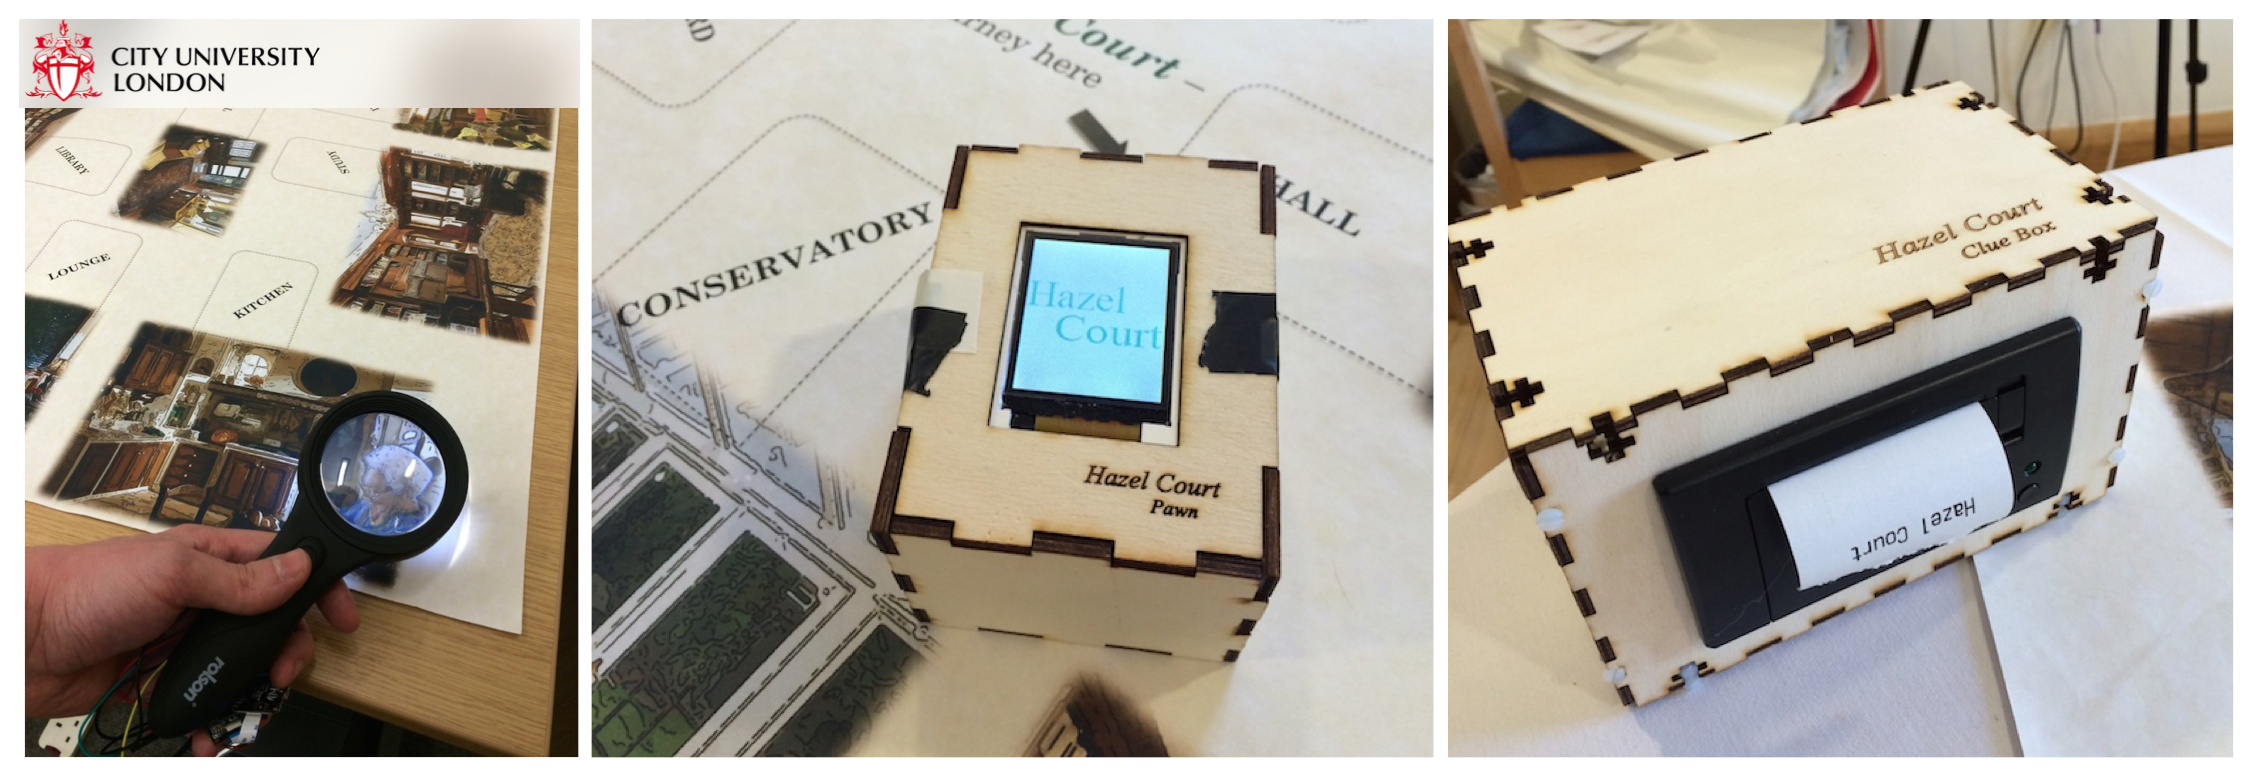
\includegraphics[width=1\textwidth]{city}
    \caption{The Hazel Court prototype}
    \label{fig:hazel-court}
\end{figure}

During twelve weeks spent as visiting fellow at the MIT SENSEable City
Lab I investigated the design and production of a tangible interface to
promote user engagement and reflection about urban-mobility data. I
worked under the supervision of professor Carlo Ratti. A working
prototype of \emph{DriveWAVE} (Figure \ref{fig:drivewave}) has been
implemented. DriveWAVE is a tangible interface that allows casual
players in public spaces to challenge a computer brain against managing
car flows towards minimizing pollution and avoiding traffic jams. The
installation aims at sparking the interest in future sustainable
cities\footnote{For more information please visit
  http://senseable.mit.edu/wave/}. The prototype features sensing-based
interaction with the audience via presence sensors, physical controllers
and digital projections. The work has been displayed to the public in
two exhibitions: ``Wave'' held in Paris and ``CNR Internet Festival''
held in Pisa, Italy. This experiences streghtned my competences in
building complex sensing-based systems to be deployed in public settings
and added to the investigation of RQ3.

\begin{figure}[h]
    \centering
    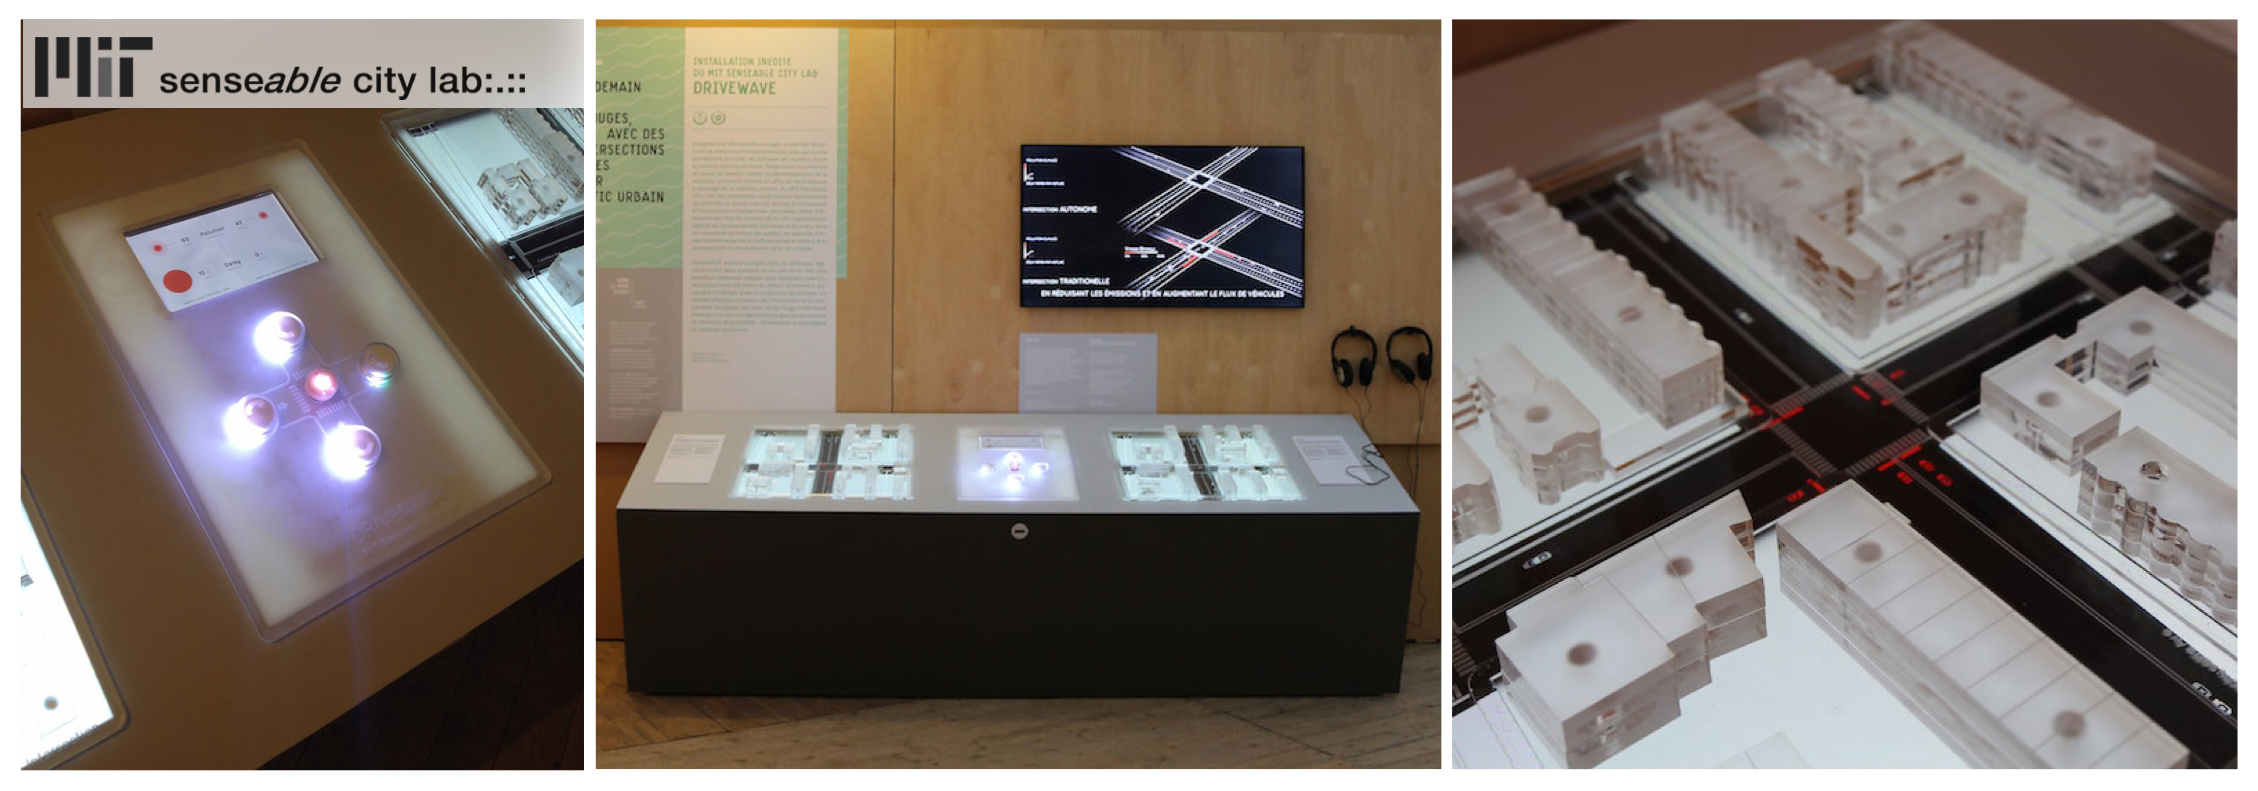
\includegraphics[width=1\textwidth]{mit}
    \caption{The DiveWAVE prototype}
    \label{fig:drivewave}
\end{figure}

I also co-advised thesis works of eight master students who have
contributed to the development of prototypes. One of them co-authored
P1.

\section{Structure of the thesis}\label{structure-of-the-thesis}

The thesis is structured as follows:

\textbf{Chapter 2} introduces the Crisis domain providing an overview on
scenarios, activities and roles; and presenting debriefing as a tool for
experiential learning.

\textbf{Chapter 3} describes relevant background theory on reflective
and experience-based learning with focus on describing the Computer
Supported Reflective Learning model adopted as theoretical underpinning
of this research work.

\textbf{Chapter 4} presents relevant background theory in sensing
based-interaction, motivating the use of that category of applied to
reflective learning.

\textbf{Chapter 5} depicts the research strategy and approach adopted by
this PhD work, giving and overview of the user studies conducted and
prototypes built.

\textbf{Chapter 6} summarises the results for the research papers.

\textbf{Chapter 7} outlines the contribution of this thesis and their
relations to the research papers.

\textbf{Chapter 8} proposes an evaluation of the work done.

\textbf{Chapter 9} concludes the thesis and sketches out future research
and innovation works.

\textbf{Appendix A} contains the research papers P1-P7.

\textbf{Appendix B} summarises secondary research papers that were
written during the research fellowship.

\textbf{Appendix C} includes a benchmark of hardware toolkits for rapid
prototyping which has been used to select the specific tools used to
implement the prototypes in this PhD.
